\documentclass[12pt, a4paper]{article}

\usepackage{array}
\usepackage[portuguese]{babel}
\usepackage{chngpage}
\usepackage{float}
\usepackage[a4paper, margin=2cm]{geometry}
\usepackage{graphicx}
\usepackage{hyperref}
\usepackage{listings}
\usepackage{setspace}
\usepackage{xcolor}

\title{\Huge \textbf{Computação Gráfica \\ \Large Trabalho Prático -- Fase I}}
\date{2 de março 2025}
\author{Grupo \textbf{\color{red} TODO}}

\begin{document}

\begin{center}
    
\includegraphics[width=0.25\textwidth]{res/cover/EE-C.eps}
\end{center}

\chardef\_=`_
\onehalfspacing
\setlength{\parskip}{\baselineskip}
\setlength{\parindent}{0pt}
\def\arraystretch{1.5}

{\let\newpage\relax\maketitle}
\maketitle
\thispagestyle{empty}

\vspace*{\fill}

\begin{adjustwidth}{-2cm}{-2cm} % These values only need to be large enough to center the table
    \begin{center}
        \begin{tabular}{>{\centering}p{0.25\textwidth}
                        >{\centering}p{0.25\textwidth}
                        >{\centering}p{0.25\textwidth}
                        >{\centering\arraybackslash}p{0.25\textwidth}}
            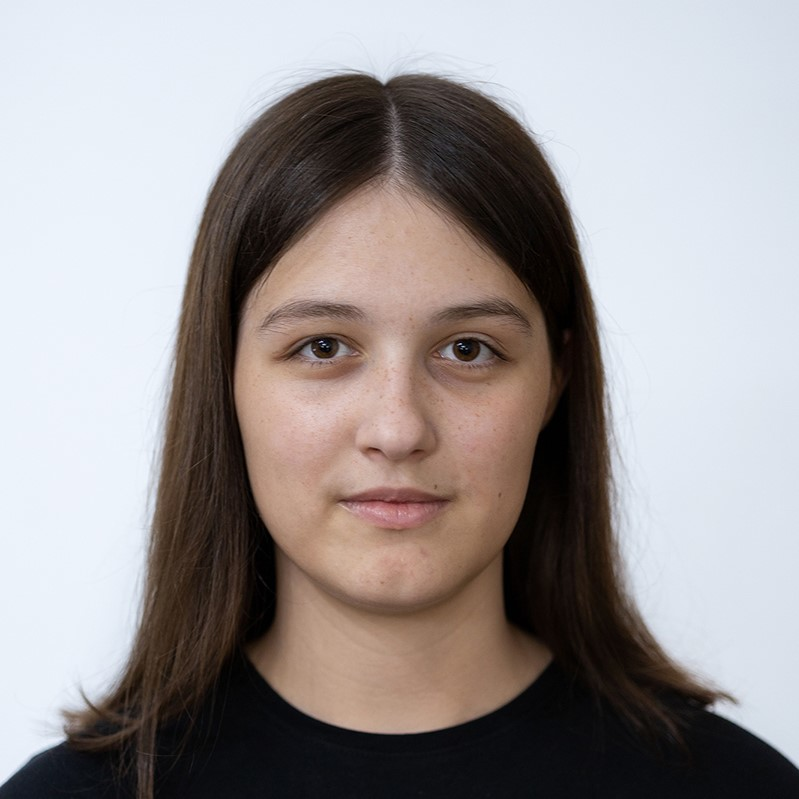
\includegraphics[width=3.5cm]{res/cover/A104437.png} &
            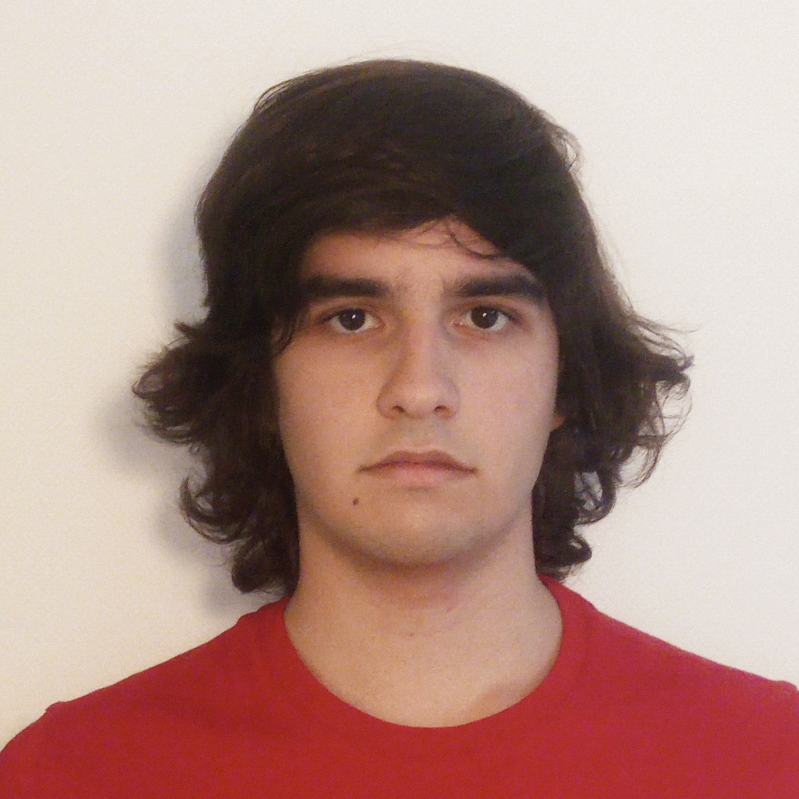
\includegraphics[width=3.5cm]{res/cover/A104348.png} &
            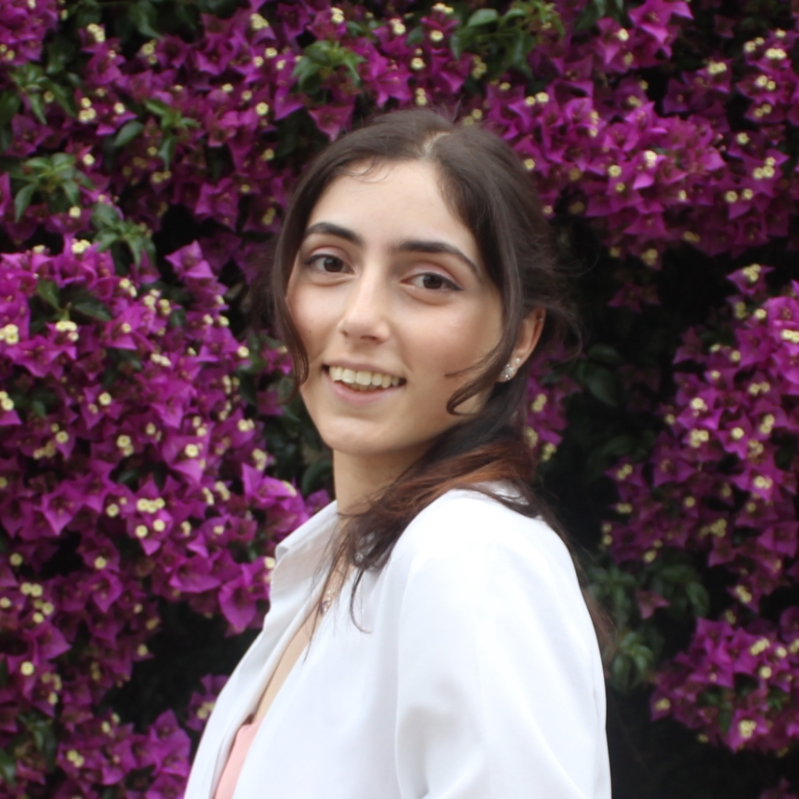
\includegraphics[width=3.5cm]{res/cover/A90817.png} &
            
\includegraphics[width=3.5cm]{res/cover/A104179.png} \\

            Ana Oliveira & Humberto Gomes & Mariana Cristino & Sara Lopes \\
            A104437      & A104348        & A90817           & A104179
        \end{tabular}
    \end{center}
\end{adjustwidth}

\pagebreak

\begin{abstract}
    \textbf{\color{red} TODO - resumo}
\end{abstract}

\section{\emph{Generator}}

\textbf{\color{red} TODO - \emph{generator}}

\section{\emph{Engine}}

\subsection{Cena (\texttt{Scene})}

A classe \texttt{Scene} assume um papel fulcral na \texttt{engine}, pois é responsável por
interpretar ficheiros XML com os conteúdos que devem ser renderizados. Para a sua análise sintática
destes ficheiros, a biblioteca \texttt{TinyXML2} \cite{tinyxml2} é utilizada. Segue um exemplo de
uma cena em formato XML:

% TODO - adjust listing style and syntax highlighting after merging

\begin{lstlisting}

<world>
    <window width="512" height="512" />
    <camera>
        <position x="3" y="2" z="1" />
        <lookAt x="0" y="0" z="0" />
        <up x="0" y="1" z="0" />
        <projection fov="60" near="1" far="1000" />
    </camera>
    <group>
        <models>
            <model file="../models/box.3d" />
        </models>
    </group>
</world>
\end{lstlisting}

O processo de análise inicia-se com a leitura do elemento raiz, \texttt{<world>}, que contêm todos
os elementos de configuração. A \texttt{Scene} começa por extrair as dimensões da janela a partir do
elemento \texttt{<window>} e as propriedades da câmara a partir do elemento \texttt{<camera>}.
Depois, prossegue à leitura dos objetos presentes na cena. Os elementos \texttt{<group>} podem
conter outros elementos \texttt{<group>}, ou então elementos \texttt{<model>}, que especificam os
modelos 3D a serem carregados e renderizados. Nesta primeira fase, por simplicidade, esta estrutura
hierárquica é linearizada durante o carregamento de uma cena (a \texttt{engine} armazena um
\texttt{std::vector} de modelos), mas isto é algo que terá de ser mudado para suportar as
transformações geométricas da próxima fase.

O leitor de cenas procura evitar o carregamento do mesmo modelo mais do que uma vez. Com recurso a
um dicionário (\texttt{std::unordered\_map}), são armazenados os modelos já carregados. Quando um
elemento \texttt{<model>} é encontrado, caso este refira um ficheiro \texttt{.3d} carregado
anteriormente, ele é reutilizado; caso contrário, um novo modelo é carregado e armazenado no
dicionário.

A classe \texttt{Scene} também é responsável por desenhar os conteúdos de uma cena. Para o fazer,
começa por configurar a matriz da câmara no \emph{shader} de vértices, e itera por todas as
entidades, desenhando cada uma.

\subsection{Entidade (\texttt{Entity})}

A classe \texttt{Entity} representa um objeto 3D individual na cena, combinando um modelo
(\texttt{Model}) com outra informação relevante como, por exemplo, a sua cor. Esta classe é também
responsável por renderizar cada objeto corretamente, transformando o seu modelo de acordo com os
atributos definidos.

Uma otimização feita à \texttt{Entity} é o uso de um \texttt{std::shared\_ptr<Model>} para
referenciar o modelo associado a cada objeto. Este apontador inteligente permite a partilha do mesmo
modelo por várias entidades que o usem, reduzindo o consumo de memória da GPU. Ademais, o uso de
contagem de referências permite a libertação automática de memória, seguindo os princípios RAII de
C++.

\section{Resultados obtidos}

\textbf{\color{red} TODO - resultados}

\section{Conclusão e Trabalho Futuro}

\textbf{\color{red} TODO - conclusão}

\begingroup
\section{Bibliografia}
\renewcommand{\section}[2]{}

\begin{thebibliography}{9}
    \bibitem{tinyxml2}
        "TinyXML-2."{} GitHub. Mar. 2, 2025. [Online.] Available:
        \url{https://github.com/leethomason/tinyxml2}
\end{thebibliography}
\endgroup

\end{document}
